\section{Experiments}
\label{sec:experiments}

%% Introduction
This section describes the robot and the set of experiments used to demonstrate the efficacy of the modeling and control methods from Sections \ref{sec:sysid} and \ref{sec:mpc}.

%% SUBS: Description of the system being 
\subsection{Robot Description: Soft Arm with Laser Pointer}
\label{sec:robot}

The robot used for the experiments is a suspended soft arm with a laser pointer attached to the end effector (see Fig. \ref{fig:rig}). 
The laser dot is projected onto a ${45\text{cm} \times 45\text{cm}}$ flat board which sits $30\text{cm}$ beneath the tip of the laser pointer when the robot is in its relaxed position (i.e. hanging straight down) \Dan{these numbers are made up need to measure}.
The position of the laser dot is measured by a digital webcam overlooking (aimed at) the board.

The arm itself consists of two sections composed of three pneumatic artificial muscles or PAMs (also known as McKibben actuators \cite{tondu2012modelling}) adhered to a central foam spine by latex rubber bands (see Fig. \ref{fig:rig}) .
The PAMs in the upper and lower sections are internally connected so that only three input pressure lines are required, and
they are arranged such that for any bending of the upper section, bending in the opposite direction occurs in the bottom section.
This ensures that the laser pointer mounted to the end effector points down toward the board at all times.
The pressures inside the actuators are regulated by three Enfield TR-010-g10-s pneumatic pressure regulators, which accept ${0-10}$V command signals corresponding to pressures of ${ \approx 0 - 140 }$ kPa.

In all the experiments the system input ${u \in \Real^{3}}$ was considered to be the voltages into the pressure regulators,
and the state ${x \in \Real^2}$ was considered to be the position of the laser dot with respect to the center of board


%% Rig figure
\begin{figure}
    \centering
    \includegraphics[width=\linewidth]{figures/rig_N_robot.pdf}
    \caption{The soft robot consists of two bending segments with a laser pointer attached to the end effector. A set of three pressure regulators is used to control the pressure inside of the pneumatic actuators (PAMs), and a camera is used to track the position of the laser dot.}
    \label{fig:rig}
\end{figure}

%% SUBS: NOISE CHARACTERIZATION
\subsection{Characterization of Stochastic Behavior}
\label{sec:noise}

An input-output system is said to exhibit \emph{stochastic} behavior if identical inputs sometimes produce different outputs.
Most mechanical systems demonstrate this behavior to some extent, which limits the predictive capability of any model.

We quantified the stochastic behavior of our soft robot system by observing the variations in output from period-to-period under sinusoidal inputs of the form
\begin{align}
    u_k &= \begin{bmatrix} 6 \sin ( \frac{2 \pi}{T} k T_s ) + 3 \vspace{5pt} \\ 
    6 \sin ( \frac{2 \pi}{T} k T_s - \frac{T}{3} ) + 3 \vspace{5pt} \\ 
    6 \sin ( \frac{2 \pi}{T} k T_s  - \frac{2T}{3}) + 3\end{bmatrix}
    \label{eq:unoise}
\end{align}
for periods of $T = 6,7,8,9,10,11,12$ seconds and a sampling time of $T_s = 0.1$ seconds with a zero-order-hold between samples. 
Under these inputs, the laser dot roughly traced out a circle, with some variability in the trajectory over each period.
In Fig. \ref{fig:noise} the trajectories over 210 periods are superimposed along with the average over all trials.
Nearly all of the observed points fell within 1 cm of the mean trajectory.
Given this inherent stochasticity, even the best controller may only have the ability to control the output to within 1 cm of a desired trajectory. \Dan{Need help rewording so it doesn't just sound like I'm trying to lower expectations before the results section}.

%% FIG: Noise inherent to the system
\begin{figure}
    \centering
    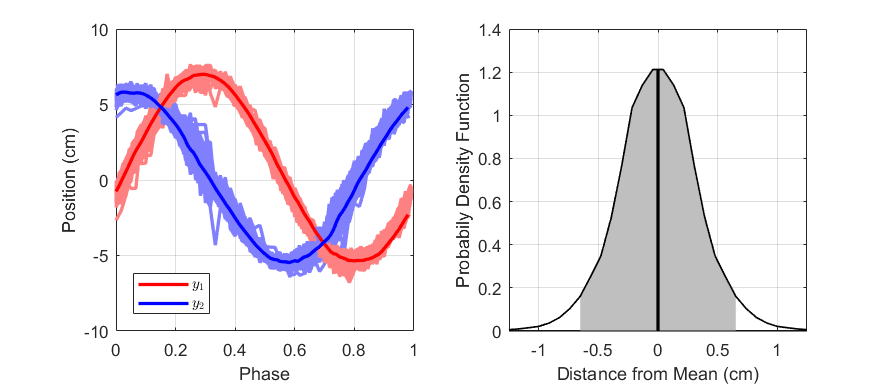
\includegraphics[width=\linewidth]{figures/noise_ph.png}
    \caption{\Dan{To be replaced with an all grey version. Any suggestions for a better label for the y-axis of the pdf?}}
    \label{fig:noise}
\end{figure}

%% SUBS: DATA COLLECTION
\subsection{Data Collection and Model Identification}
\label{sec:datacollection}

% How data was collected
Data collection proceeded in 16 trials, each lasting roughly 20 minutes \Dan{double check}.
To generate a representative sampling of the system's behavior over its entire operation range, a randomized input was applied during each trial.
Beforehand, a $3 \times 1000$ table $\Upsilon$ of uniformly distributed random numbers between zero and ten was generated to be used as an input lookup table.
Each control input was smoothly varied between elements in consecutive columns of the table over a transition period $T_u$, with a time offset of $T_u / 3$ between each of the three control signals
\begin{align}
    u_i (t) &= \frac{(\Upsilon_{i,k+1} - \Upsilon_{i,k})}{T_u} \left( t + \frac{(i-1) T_u}{3} \right) + \Upsilon_{i,k}
    \label{eq:input}
\end{align}
where $k = \text{floor}\left( {t} / {T_u} \right)$ is the current index into the lookup table at time $t$. 
The transition period $T_u$ varied from 5 seconds to 8 seconds between trials \Dan{double check}.
After collection, the data was uniformly sampled with period $T_s = 0.1$ s.

% Models were build from this data
Two models were fit from the data: a linear Koopman model, and a linear state space model.
The linear state-space model, intended to provide a baseline of comparison, was identified from the same data as the Koopman model using the Matlab System Identification Toolbox \cite{MATLAB:2017}.
This model is a four dimensional linear state space model expressed in observability canonical form.

The Koopman model was identified via the method described in Section \ref{sec:sysid} on snapshot pairs $\{ a_k , b_k \}$ incorporating a single delay $d = 1$
\begin{align}
    a_k &= \begin{bmatrix} x_k^\top , & x_{k-1}^\top , & u_{k-1}^\top \end{bmatrix}\top \\
    b_k &= \begin{bmatrix} \left( \phi_{T_s} (x_k) + \sigma_k \right)^\top, & x_{k}^\top, & u_{k}^\top \end{bmatrix}^\top,
\end{align}
and using the $N=330$ dimensional set of basis functions consisting of all monomials of maximum degree 4.
To find the sparsest acceptable matrix representation of the Koopman operator, equation \eqref{eq:lasso} was solved for ${ \lambda = 0.1 k}$ where ${k = 0,1, ... , 50 }$.
Predictions from the resulting models were evaluated against a subset of the training data, with the error quantified as the average Euclidean distance between the prediction and actual trajectory at each point.
Fig. \ref{fig:lasso} shows that as $\lambda$ increases so does this error, but the density of the $A$ matrix of the lifted linear model decreases.
The model chosen is the one that minimizes both density and prediction error.

%% FIG: MODEL VS. WEIGHT OF L1 PENALTY (LASSO)
\begin{figure}
    \centering
    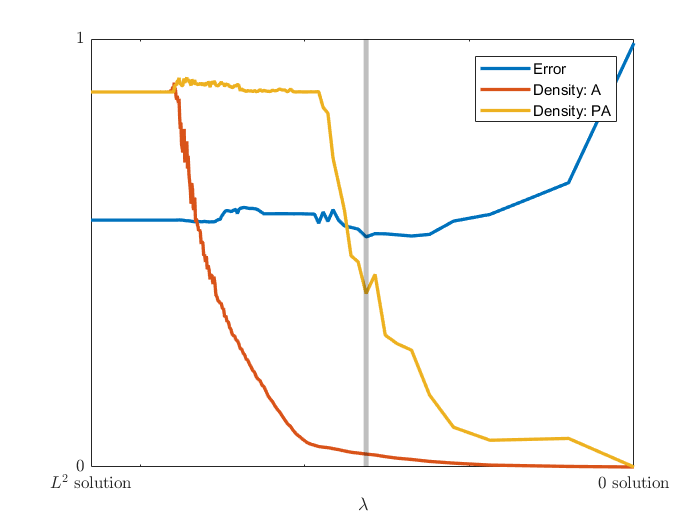
\includegraphics[width=\linewidth]{figures/lasso_ph.png}
    \caption{\Dan{Ram I am going to replace this with one from the training data. You're right that it is weird to include the fake example.} As the weight of the L1 penalty term increases, the Koopman operator matrix becomes more dense, and the model error decreases then levels off. This shows that there is a much sparser representation of the Koopman operator than the least-squares solution that generates a model of nearly identical accuracy.}
    \label{fig:lasso}
\end{figure}


%% SUBS: PREDICTOR COMPARISON
\subsection{Experiment 1: Model Prediction Comparison}
\label{sec:predict}

The accuracy of the predictions generated by each of the two models were evaluated by comparing them to the actual behavior of the system under the sinusoidal inputs described in Section \ref{sec:noise}.
The model responses were simulated over a time horizon of 2.5 seconds given the same initial condition and input as the real system.
The results of this comparison are summarized by Fig. \ref{fig:predict} and Table \ref{tab:predict}, which show that the Koopman model predictions are more accurate over the time horizon.

%% FIGURE: Linear vs. Koopman model predictions
\begin{figure}
    \centering
    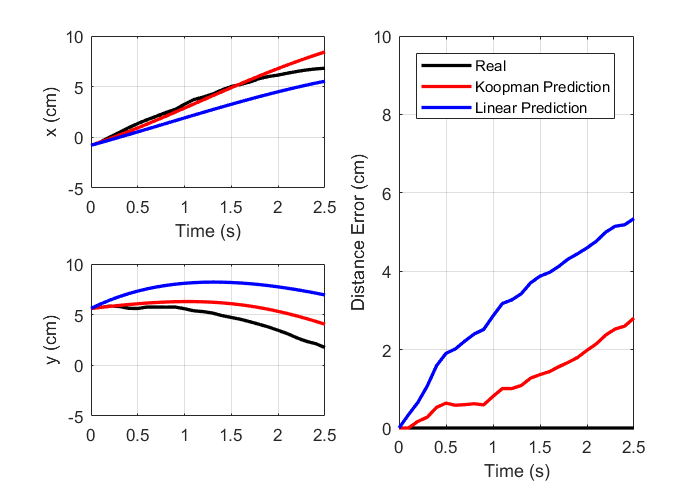
\includegraphics[width=\linewidth]{figures/predictionComparison_ph.png}
    \caption{\Dan{Placeholder for plot showing the prediction comparison between the koopman and the linear state space model.}}
    \label{fig:predict}
\end{figure}




%% SUBS: Description of the controllers and tracing task
\subsection{Experiment 2: Model-Based Control Comparison}
\label{sec:mpcexp}
\Dan{Lot's of imprecise explanations in this section}

%% Description of compared controllers
Each of the identified models was used to build a model predictive controller which solves an optimization problem in the form of \eqref{eq:mpc} at each time step.
We refer to each of the controllers by the abbreviations K-MPC for the one based on the Koopman model, and L-MPC for the one based on the linear state-space model.
Both model predictive controllers run in closed-loop at $10$ Hz, feature an MPC horizon of 2.5 seconds ($N_h = 25$), and a cost function that penalizes deviations from an output reference trajectory $r_{[k]}$ over the horizon with both a running and terminal cost:
\begin{align}
    \text{cost} &= 100 (C z_{[N_h]} - r_{[N_h]})^2 + \sum_{i=0}^{N_h - 1} 0.1 (C z_{[i]} - r_{[i]})^2
\end{align}
where $z$ signifies the $N=625$ dimensional \emph{lifted state} $\psi(y)$ in the K-MPC case, and the $n=4$ dimensionsal state $x$ in the L-MPC case, and $C$ is the projection matrix corresponding to each.

% The optimization problem for each controller also featured a convex constraint to limit the rate at which the control inputs could change over time... 

% task
The performance of the controllers was assessed with respect to a set of two trajectory following tasks.
Each task was to follow a reference trajectory as it traced out the following shapes:
\begin{enumerate}
    \item Block letter M (see Fig. \ref{fig:compare_blockM})
    \item Pacman (see Fig. \ref{fig:compare_pacman})
\end{enumerate}
The error for each trial was quantified as the Cartesian distance from the desired point at each time step over the length of the trial.

The performances of the K-MPC and L-MPC controllers at Tasks 1 and 2 is shown visually in Fig. \ref{fig:compare_blockM} and \ref{fig:compare_pacman}, and the error is quantified in Table \ref{tab:RMSE}.
In both tasks the K-MPC controller performed best, exhibiting an average tracking error of --- cm which is --- cm lower than that of the L-MPC controller.



%% FIGURE: Visual comparison of controller performance for the block M.
\begin{figure*}
    \centering
    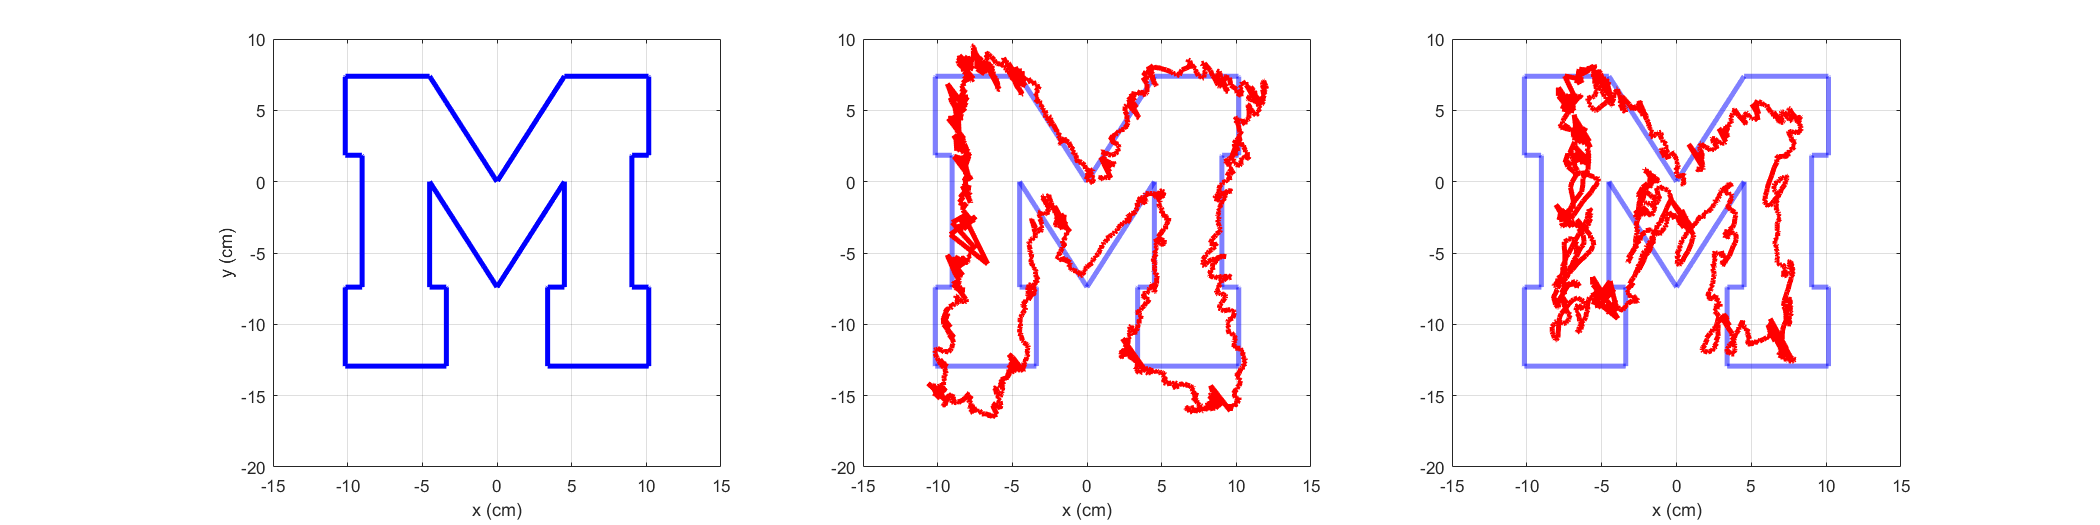
\includegraphics[width=\linewidth]{figures/compare_blockM_300s_draft.png}
    \caption{The results of each controller to performing task 1. Reference trajectory only (left). Koopman MPC (middle). Linear MPC (right). Laser dot trajectory is shown in red, the reference trajectory is shown in blue.}
    \label{fig:compare_blockM}
\end{figure*}

%% FIGURE: Visual comparison of controller performance for the pacman.
\begin{figure*}
    \centering
    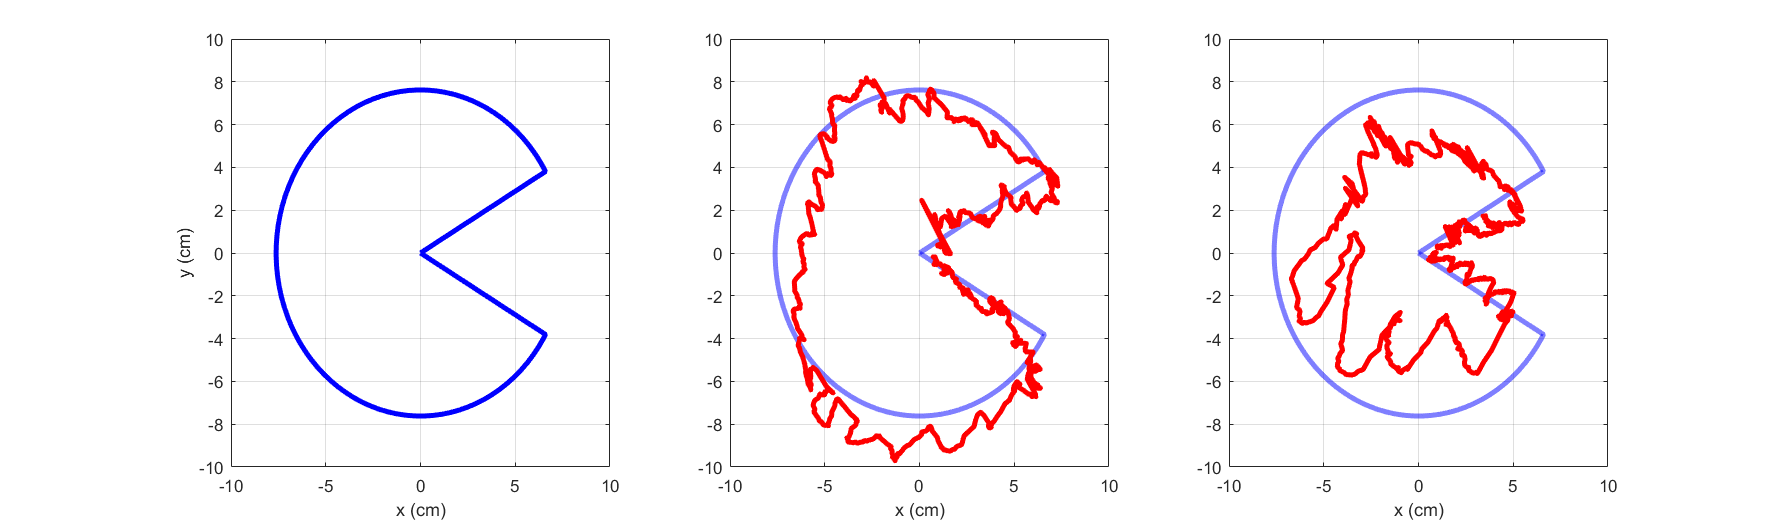
\includegraphics[width=\linewidth]{figures/compare_pacman68_90s_draft.png}
    \caption{The results of each controller to performing task 2. Reference trajectory only (left). Koopman MPC (middle). Linear MPC (right). Laser dot trajectory is shown in red, the reference trajectory is shown in blue.}
    \label{fig:compare_pacman}
\end{figure*}

%% TABLE: RMSE results table
\begin{table}[]
    \rowcolors{2}{white}{gray!25}
    \setlength\tabcolsep{5pt} % default value: 6pt
    \centering
    \caption{RMSE (cm) over all trajectory following tasks \Dan{Fill in real results later}}
    \begin{tabular}{|c|c|c|c|c|c|c|c|c|}
        \hline
        \rowcolor{white} 
        & \multicolumn{6}{c |}{\textbf{Task}} & & \textbf{Std.} \\
        \cline{2-7} \rowcolor{white}
        \multirow{-2}{*}{\textbf{Controller}} & $1$ & $2$ & $3$ & $4$ & $5$ & $6$ & \multirow{-2}{*}{\textbf{Avg.}} & \textbf{Dev.} \\
        \hline
        % RESULTS FOR ROBOT A
        Koopman MPC &  2.4  &  2.0  &  2.9  &  1.7  &  1.5  &  2.0 & 2.1 & 0.5 \\
        Linear MPC  &  5.8  &  4.0  &  6.6  &  3.9  &  2.8  &  3.5 & 4.5 & 1.5 \\
        Nonlinear MPC &  5.1  &  3.1  &  9.9  &  3.0  &  1.8  &  4.8 & 4.6 & 2.9 \\
        % Ham.-Weiner &  7.0  &  4.5  &  6.9  &  3.0  &  2.3  &  3.1 & 4.5 & 2.0 \\
        % \multirow{-5}{*}{\cellcolor{white} \rotatebox[origin=c]{90}{\textbf{Robot A}}}
        % NLARX       &  5.0  &  3.0 &  12.0  &  3.8  &  2.1  &  2.8 & 4.8 & 3.7 \\
        \hline
        % % RESULTS FOR ROBOT B
        % \cellcolor{white} & Koopman & & & & & & & & \\
        % \cellcolor{white} & Neural Net & & & & & & & & \\
        % \cellcolor{white} & State Space & & & & & & & & \\
        % \cellcolor{white} & Ham.-Weiner & & & & & & & & \\
        % \multirow{-5}{*}{\cellcolor{white} \rotatebox[origin=c]{90}{\textbf{Robot B}}}
        % & NLARX & & & & & & & & \\
        % \hline
    \end{tabular}
    \label{tab:RMSE}
\end{table}